\begin{problem}[Initial Value Problem With Cross Product]\label{prb:cross-prod} 


%%%%%%%%%%%%%%%%%%%%%%%%%%%%%%%%%%%%%%%%%%%%%%%%%%%%%%%%%%%%%%%%%%%%%%%%%%
% INSTEAD OF COMMENTING OUT SUBPROBLEMS, USE \hidesubprb,
% so the subproblem is still displayed in the catalogue!
%%%%%%%%%%%%%%%%%%%%%%%%%%%%%%%%%%%%%%%%%%%%%%%%%%%%%%%%%%%%%%%%%%%%%%%%%%

We consider the initial value problem
\begin{equation}
  \label{eq:awp3}
  \dot{\Vy} = \Vf(\Vy) := \Va\times\Vy + c\Vy\times(\Va\times\Vy),\quad
  \Vy(0) =\Vy_0 =  [1,1,1]^\top,
\end{equation}
where $c>0$ and $\Va\in\bbR^3$, $\norm{a}_2 = 1$.

NOTE: $\Vx\times\Vy$ denotes the cross product between the vectors $\Vx$ and $\Vy$. It is defined by
\[
\Vx\times\Vy = [x_2 y_3 -x_3 y_2 , x_3y_1 - x_1 y_3,x_1y_2 - x_2 y_1]^\top. 
\]
It satisfies $\Vx\times\Vy \,\bot\, \Vx$. In Eigen, it is available as \texttt{x.cross(y)}.



\begin{subproblem}[2]\label{sp:existence}
Show that $\norm{\Vy(t)}_2=\norm{\Vy_0}_2$ for every solution $\Vy$ of~\eqref{eq:awp3}.
\begin{hint}
Target the time derivative $\frac{d}{dt}\norm{\Vy(t)}_2^2$ and use the product rule.
\end{hint}
\begin{solution}
    We have
    \begin{align*}
      &\left(\Va\times\Vy + c(\Vy\times(\Va\times\Vy))\right)\cdot\Vy = 0\\
      &\Rightarrow D_{t}\norm{\Vy(t)}_2^2 =2 \dot{\Vy}(t)\cdot\Vy(t) =
      0\\
      &\Rightarrow \norm{\Vy(t)}_2^2 = \text{const. }\forall t.
    \end{align*}
    Thus $\norm{\Vy(t)}_2=\norm{\Vy(0)}_2=\norm{\Vy_0}_2$.
\end{solution}
\end{subproblem}

\begin{subproblem}[3]
Compute the Jacobian $D\Vf(\Vy)$. Compute also the spectrum $\sigma(D\Vf(\Vy))$ in the stationary state $\Vy=\Va$, for which $\Vf(\Vy)=0$. For simplicity, you may consider only the case $\Va=[1,0,0]^\top$.
\begin{solution}
Using the definition of cross product, a simple but tedious calculation shows that
\[
D\Vf(\Vy)=
\begin{bmatrix}
-ca_2 y_2  - ca_3 y_3  &  -a_3 +2ca_1y_2 - c a_2 y_1   &    a_2-ca_3 y_1 + 2ca_1 y_3  \\
a_3-ca_1y_2+2ca_2y_1   &   -ca_3y_3-ca_1y_1  &   -a_1+2ca_2y_3-ca_3y_2  \\
-a_2+2ca_3y_1-ca_1y_3  &  a_1 - ca_2y_3 + 2ca_3  y_2  &  -ca_1y_1 - ca_2y_2
\end{bmatrix}
.
\]
Thus for $\Vy=\Va$ we obtain
\[
D\Vf(\Va)=
\begin{bmatrix}
-c(a_2^2 + a_3^2)  &  -a_3 +ca_1a_2    &    a_2+ca_3 a_1   \\
a_3+ca_1a_2   &   -c(a_1^2+a_3^2)  &   -a_1+ca_2a_3  \\
-a_2+ca_1a_3  &  a_1 + ca_2a_3   &  -c(a_1^2+a_2^2)
\end{bmatrix}
.
\]
A direct calculation gives that the spectrum is given by
\[
\sigma(D\Vf(\Va)) = \{0,-c\norm{a}_2^2 \pm i \norm{a}_2\}=\{0,-c \pm i \}.
\]
Therefore, the problem is stiff for large $c$ (see \lref{emph:stiff}).
\end{solution}
\end{subproblem}

\begin{subproblem}[2]\label{sp:numofsteps}
For  $\Va=[1,0,0]^\top$,  \eqref{eq:awp3} was solved with the standard \matlab{} integrators \texttt{ode45} and \texttt{ode23s} up to the point
  $T=10$ (default Tolerances). Explain the different dependence of the total number of steps from the parameter $c$ observed in Figure~\ref{fig:a3}.
  
    \begin{figure}[!htb]
      \centering
      % stiffrotpend.eps generated with m/a3/non-exam/largec.m
      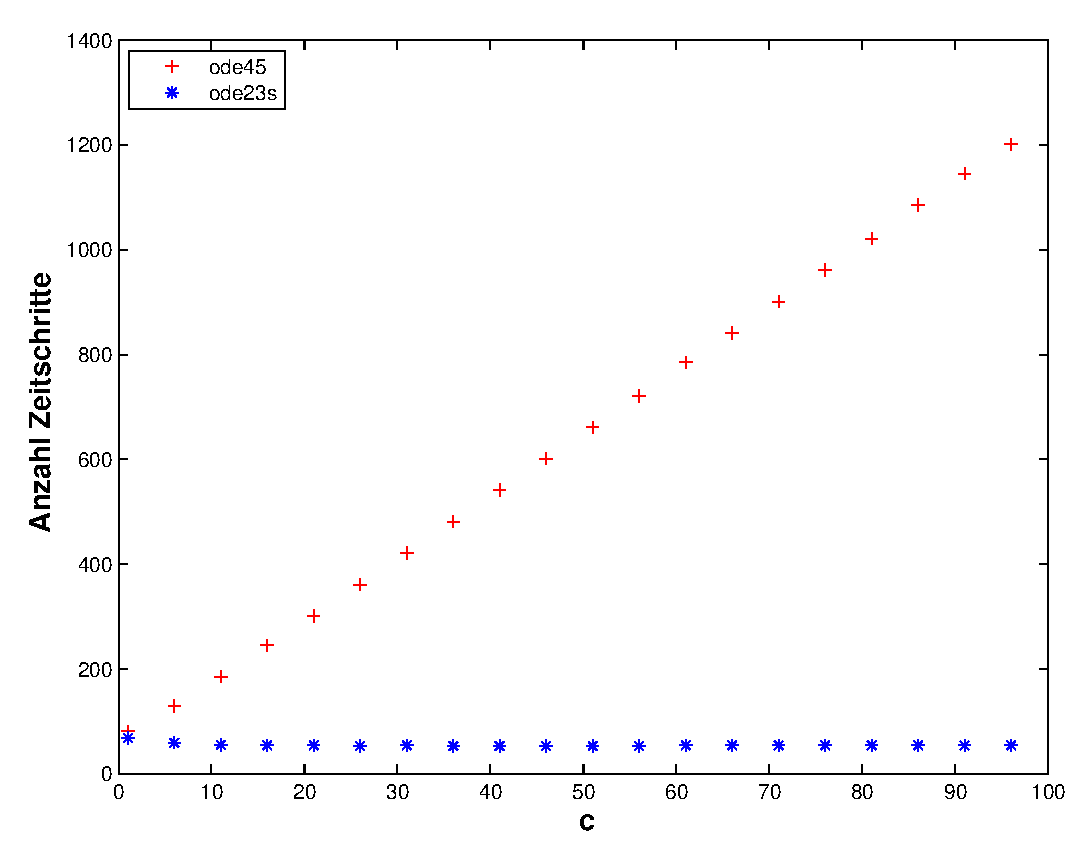
\includegraphics[width=0.9\textwidth]{../Problems/ch_ode/PICTURES/stiffrotpend.eps}
      \caption{Subproblem \ref{sp:numofsteps}: number of steps used by standard \matlab{} integrators in relation to the parameter $c$.}
        \label{fig:a3}
    \end{figure}
    
\begin{solution}
In the plot, we see that, for the solver \texttt{ode45}, the number of steps rises with $c$. On the other hand, \texttt{ode23s} uses roughly the same amount of steps, irregardless of the value of $c$ chosen.

As \texttt{ode45} is an explicit solver, it suffers under stability-based step-size limits for large $c>0$. The implicit solver \texttt{ode23s} must however not take smaller step-sizes to satisfy the tolerance for big $c$. In other words: the problem becomes stiffer, the greater the parameter $c$ is. This is expected from what we saw above.
\end{solution}
\end{subproblem}

\begin{subproblem}[2]\label{sp:4}
Formulate the non-linear equation given by the implicit mid-point rule
for the initial value problem \eqref{eq:awp3}.

\begin{solution}
With the formula for the implicit mid-point rule
    \begin{equation*}
      \Vy_{k+1} = \Vy_k + h\Vf\left(\frac{\Vy_{k} + \Vy_{k+1}}{2}\right)
    \end{equation*}
    the formulation of \eqref{eq:awp3} is given as
    \begin{equation*}
      \frac{ \Vy_{k+1} - \Vy_{k}}{h} = \Va\times\left(\frac{\Vy_k+\Vy_{k+1}}{2}\right) +
      c\left(\frac{\Vy_k+\Vy_{k+1}}{2}\right)\times\left(\Va\times\left(\frac{\Vy_k+\Vy_{k+1}}{2}\right)\right)
    \end{equation*}
\end{solution}
\end{subproblem}

\begin{subproblem}[2]
Solve \eqref{eq:awp3} with $\Va=[1,0,0]^\top$, $c=1$ up to $T=10$. Use the implicit mid-point rule and the class developed for \ref{prb:implicit_RK} with $N=128$ timesteps (use the template \texttt{cross\_template.cpp}).  Tabulate $\norm{\Vy_k}_2$ for the sequence of approximate states generated by the implicit midpoint method. What do you observe?
\begin{solution}
See file \texttt{cross.cpp}. As expected from \ref{sp:existence}, the norm of the approximate states is constant.
\end{solution}
\end{subproblem}

\begin{subproblem}[3] \label{sp:lin-imp-mpr}
The linear-implicit mid-point rule can be obtained
by a simple linearization of the incremental equation of the implicit mid-point rule around the current solution value.

Give the defining equation of the linear-implicit mid-point rule for the general autonomous differential equation
  \begin{gather*}
    \dot{\Vy} = \Vf(\Vy)
  \end{gather*}
  with smooth $f$.
  
\begin{solution}
The linear implicit mid-point rule is obtained by developing the increment $\Vk_1$ of the implicit mid point rule by its Taylor series
    \begin{align*}
      \Vk_1 = f \left(\Vy_k+\frac{h}{2}\Vk_1\right)
      = \Vf(\Vy_k) + \frac{h}{2}D\Vf(\Vy_k)\Vk_1 + O(h^2)
    \end{align*}
    and only taking the linear terms. Since the non-linear method is given by $\Vy_{k+1} = \Vy_k + h\Vk_1$, the linearization reads
    \begin{align*}
       \Vy_{k+1} = \Vy_k + h\Vk_1^{\text{lin.}}, \qquad  \Vk_1^{\text{lin.}} :=
      \left(I-\frac{h}{2}D\Vf(\Vy_k)\right)^{-1}\Vf(\Vy_k).
    \end{align*}
\end{solution}
\end{subproblem}

\begin{subproblem}[3]\label{sp:solve}
Implement the linear--implicit midpoint rule using the template provided in \texttt{cross\_template.cpp}.
Use this method to solve \eqref{eq:awp3} with $\Va=[1,0,0]^\top$, $c=1$ up to $T=10$ and $N=128$. Tabulate $\norm{\Vy_k}_2$ for the sequence of approximate states generated by the linear implicit midpoint method. What do you observe?
\begin{solution}
See file \texttt{cross.cpp}. The sequence of the norms is not exactly constant: this is due to the approximation introduced with the linearization.
\end{solution}
\end{subproblem}
\end{problem}


%%%%%%%%%%%%%%%%%%%%%%%%%%%%%%%%%%%%%%%%%%%%%%%%%%%%%%%%%%%%%%%%%%%%%%%%%%

